\chapter{Testes}  
\label{chap: testes}

\section{Dummy text com figura}

Lorem ipsum dolor sit amet, consectetuer adipiscing elit. Aenean commodo ligula eget dolor. Aenean massa. Cum sociis natoque penatibus et magnis dis parturient montes, nascetur ridiculus mus. Donec quam felis, ultricies nec, pellentesque eu, pretium quis, sem. Nulla consequat massa quis enim. Donec pede justo, fringilla vel, aliquet nec, vulputate eget, arcu. In enim justo, rhoncus ut, imperdiet a, venenatis vitae, justo. Nullam dictum felis eu pede mollis pretium.

Lorem ipsum dolor sit amet, consectetuer adipiscing elit. Aenean commodo ligula eget dolor. Aenean massa. Cum sociis natoque penatibus et magnis dis parturient montes, nascetur ridiculus mus. Donec quam felis, ultricies nec, pellentesque eu, pretium quis, sem. Nulla consequat massa quis enim. Donec pede justo, fringilla vel, aliquet nec, vulputate eget, arcu. In enim justo, rhoncus ut, imperdiet a, venenatis vitae, justo. Nullam dictum felis eu pede mollis pretium.

\begin{figure}[ht]
  \caption{Mãe, eu formei!}
  \label{fig: fig1}
  \centering
  
\includegraphics[width=0.7\textwidth]{graduation.png}
  \legend{Google images}
  
\end{figure}

\begin{figure}[ht]
  \caption{Ferramentas utilizadas}
  \label{fig: fig2}
  \centering
  \subfloat[overleaf\label{subfig: fig2a}]{
\includegraphics[width=0.3\textwidth]{overleaf.png}}
  \hfill
  \subfloat[latex\label{subfig: fig2b}]{
\includegraphics[width=0.3\textwidth]{latex.png}}
  \hfill
  \subfloat[github\label{subfig: fig2c}]{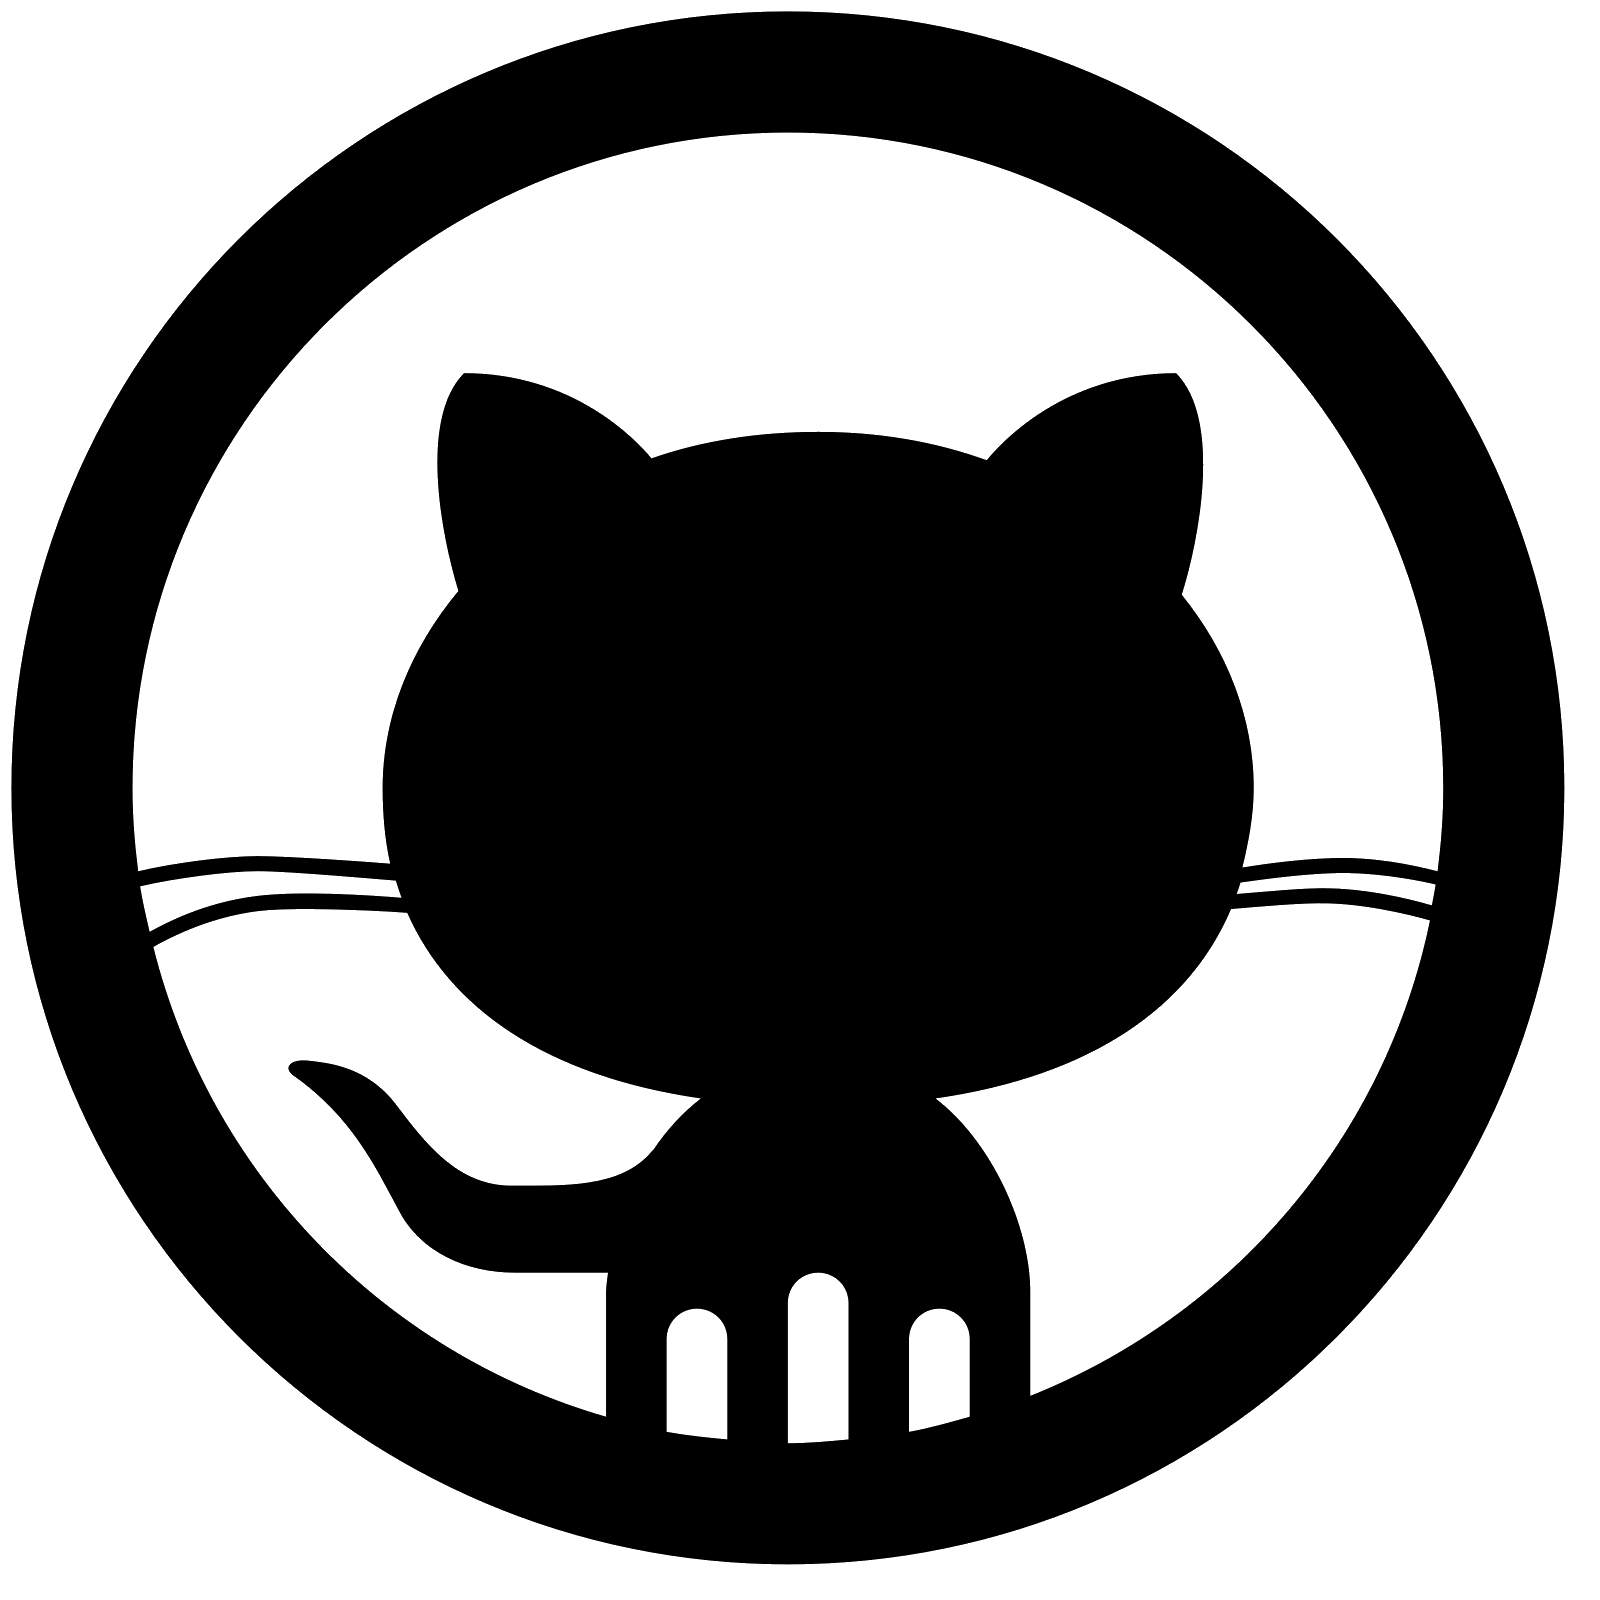
\includegraphics[width=0.3\textwidth]{github.png}}
  \legend{Google images}
  
\end{figure}

Integer tincidunt. Cras dapibus. Vivamus elementum semper nisi. Aenean vulputate eleifend tellus. Aenean leo ligula, porttitor eu, consequat vitae, eleifend ac, enim. Aliquam lorem ante, dapibus in, viverra quis, feugiat a, tellus. Phasellus viverra nulla ut metus varius laoreet. Quisque rutrum. Aenean imperdiet. Etiam ultricies nisi vel augue. Curabitur ullamcorper ultricies nisi. Nam eget dui. Etiam rhoncus. Maecenas tempus, tellus eget condimentum rhoncus, sem quam semper libero, sit amet adipiscing sem neque sed ipsum. Nam quam nunc, blandit vel, luctus pulvinar, hendrerit id, lorem. Maecenas nec odio et ante tincidunt tempus. Donec vitae sapien ut libero venenatis faucibus. Nullam quis ante. Etiam sit amet orci eget eros faucibus tincidunt. Duis leo. Sed fringilla mauris sit amet nibh. Donec sodales sagittis magna. Sed consequat, leo eget bibendum sodales, augue velit cursus nunc,

\subsection{Tabelas e Quadros}

Segue exemplos de como usar tabelas e quadros.

\begin{table}[ht]
  \caption{Faixa etária dos alunos (número e proporção) do Curso de Saneamento do Ifes – Campus Vitória no no de 2016.}
  \label{tab: table1}
  \centering

  \begin{tabular}{ccc}
    \hline
    \bfseries Faixa Etária & \bfseries Número & \bfseries Porcentagem\\
    \hline
    18 a 25 & 7 & 25,7 \\
    26 a 30 & 25 & 70,3 \\
    31 a 40 & 2 & 3,0 \\
    40 a 50 & 1 & 1,0 \\
    + de 50 & - & - \\
    \hline
    Total & 35 & 100 \\
    \hline
  \end{tabular}

  \source
\end{table}
  
\begin{quadro}[ht]
  \caption{Configuração de microcomputador XP.}
  \label{quad: quadro1}
  \centering
  
  \begin{tabularx}{\textwidth}{lX}
    \hline
    \bfseries Elemento & \bfseries Especificações\\
    \hline
    1 CD & CD + Disk Driver para apenas uma entrada de disquete \\
    Kit de multimídia 8X & Kit com placa de som, caixas, microfone, CD-ROM com velocidade 8X e títulos \\
    8 Mb RAM & Quantidade de memória RAM (ver memória) \\
    66 Mhz & Velocidade do computador \\
    PC 486 DX/2 & Tipo e modelo do computador \\
    840 Mb HD & Capacidade de armazenamento do computador \\
    \hline
  \end{tabularx}

  \legend{Barbosa (1999 apud UFES, 2004)}
\end{quadro}

\subsubsection{Teste com referências}

Segue abaixo uma lista de referências:

\begin{itemize}%[nosep]
  \item Citando os autores: \citeonline{Goodfellow2016}
  \item Citando artigo/livro: \cite{Ciresan2012,SMIRNOV201489}
  \item Citando normas: \cite{NBR6023:2000}
  \item Referência cruzada com capítulos: \autoref{chap: testes}
  \item Referência cruzada com anexos: \refanexo{anexo: a}
  \item Referência cruzada com apêndices: \refapendice{apendice: a}
  \item Referência cruzada com figuras: \autoref{fig: fig1}
  \item Referência cruzada com sub-figuras: Figura \ref{subfig: fig2a}
  \item Referência cruzada com tabelas: \autoref{tab: table1}
  \item Referência cruzada com quadros: \autoref{quad: quadro1}
  \item Referência cruzada com equações: \autoref{eq: eq1}
\end{itemize}
    
\subsubsubsection{Equações e Códigos}

O Teorema de Pitágoras é dado por:

\begin{equation}
    \label{eq: eq1}
	a^{2}= b^{2}+c^{2}
\end{equation}

Exemplo de código de programação:
  
\lstinputlisting[language=Python, caption=Perceptron]{algoritmos/perceptron.py}